% KAJIAN PUSTAKA 1
\begin{frame}
    \begin{columns}
        \begin{column}{0.35\textwidth}
            \LARGE
            Kajian Pustaka 1
        \end{column}
        \begin{column}{0.6\textwidth}
            \justifying
            \textbf{Judul:}\\
            Extended Kalman Filter (EKF) design for vehicle position tracking using reliability function of Radar and Lidar

            \vspace{1.5em}

            \textbf{Penulis:}\\
            Kim, Taeklim; Park, Tae-Hyoung

            \vspace{1.5em}
            
            \textbf{Publikasi:}\\
            MDPI Sensors, vol.20, no.15, p.4126, 2020
        \end{column}
    \end{columns}
\end{frame}


\begin{frame}
    \frametitle{Pustaka 1: Pendahuluan}
    \large
    \begin{itemize}
        \justifying
        \item Desain Extended Kalman Filter untuk menggabungkan data Lidar dan Radar
        \vspace{1em}
        \item Menghasilkan algoritma yang mampu meningkatkan akurasi dibandingkan dengan hanya menggunakan satu macam sensor.
    \end{itemize}
\end{frame}


\begin{frame}
    % \frametitle{Pustaka 1: Skema Sistem}
    \centering
    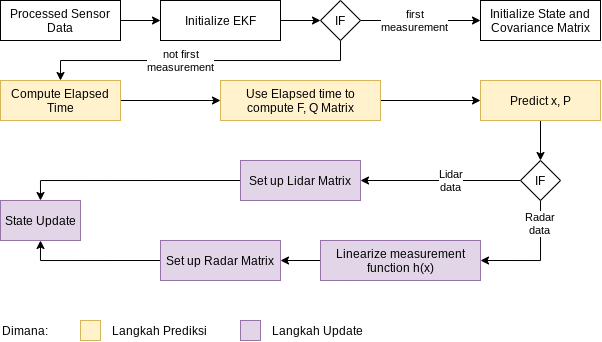
\includegraphics[width=.9\textwidth]{2-LREKF-diagram.png}
\end{frame}


\begin{frame}
    \frametitle{Pustaka 1: Metode}
    \begin{enumerate}
        \justifying
        \item Pra-proses penggabungan dilakukan menggunakan algoritma clustering dan asosiasi, dan menghasilkan centroid dari setiap objek halangan.
        \item Pada pengukuran pertama, inisialisasi state dan matriks kovarian 
        \item Prediksi dengan:
        \begin{itemize}
            \item Menghitung perubahan waktu
            \item Menghitung matriks state $F$ \& matriks kovarian $Q$ baru berdasar perubahan waktu
            \item Propagasi state $x$ \& kovarian $P$
        \end{itemize} 
        \item Bila data Radar, linearisasi fungsi pengukuran
        \item Update state dengan pengukuran dan state $x$ baru.
        \item Tracking dengan hungarian Algorithm
    \end{enumerate}
\end{frame}


\begin{frame}
    \frametitle{Pustaka 1: Hasil}
    \centering
    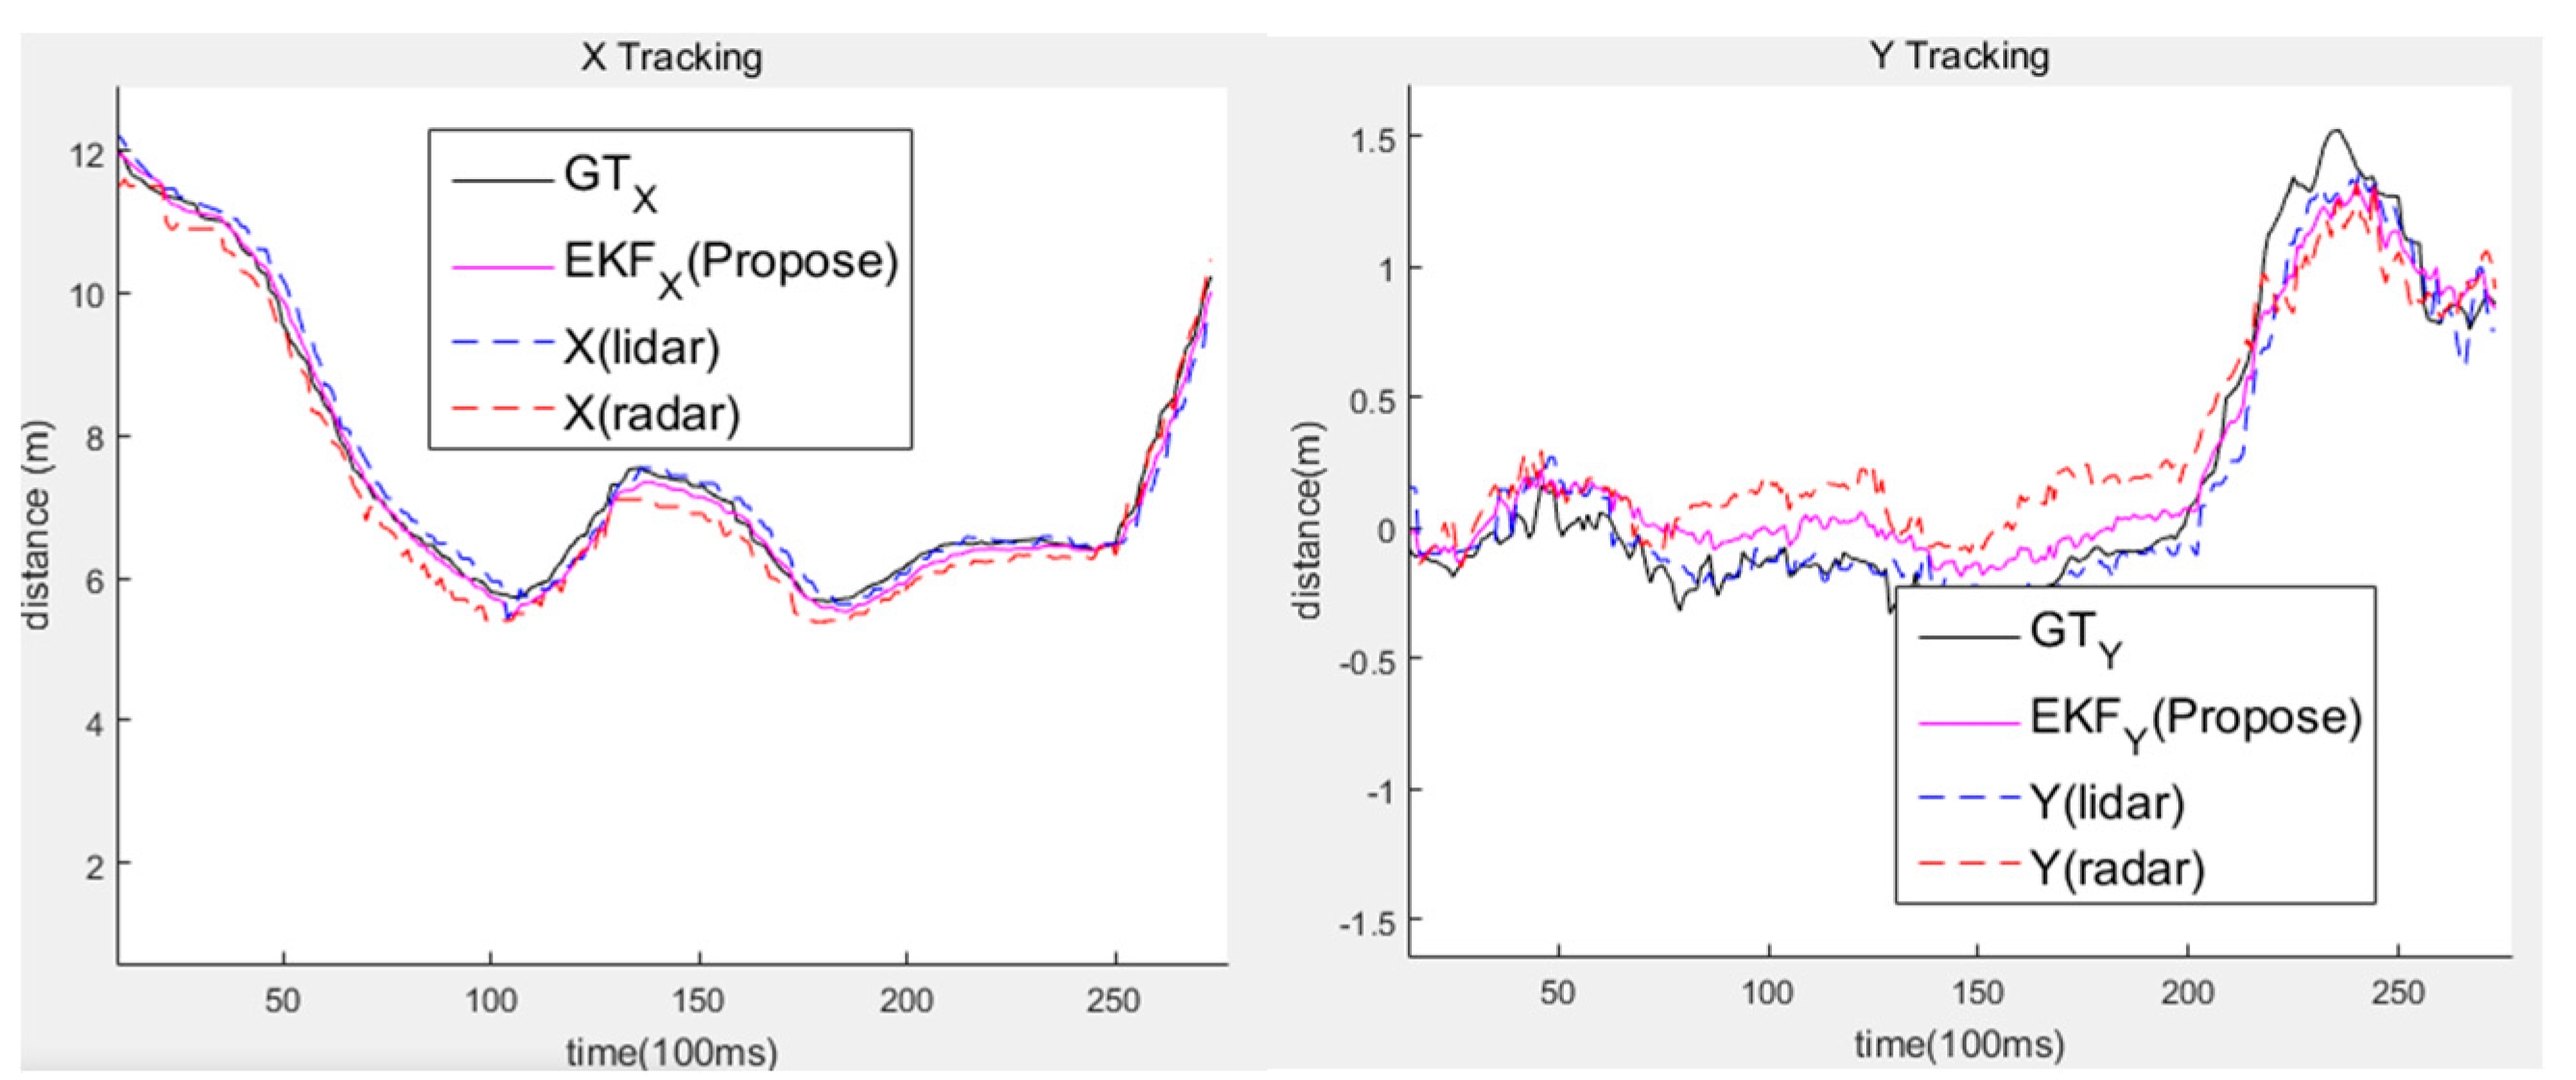
\includegraphics[width=.8\textwidth]{r1-hasil-1.png}\\
    dimana GT: Ground Truth, EKF: Algoritma EKF
\end{frame}


\begin{frame}
    \frametitle{Pustaka 1: Hasil}
    \centering
    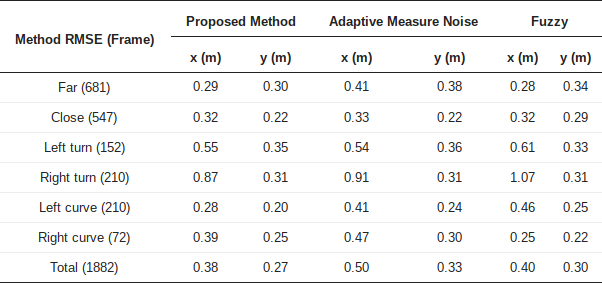
\includegraphics[width=.8\textwidth]{r1-hasil-2.png}
\end{frame}


\begin{frame}
    \frametitle{Pustaka 1: Kesimpulan}

    \large
    \textbf{Kelebihan}\\
    \normalsize
    \begin{itemize}
        \item Sensor Fusion Lidar dan Radar menggunakan algoritma ini lebih baik dibandingkan Adaptive Measure Noise dan Metode Fuzzy.
    \end{itemize}

    \large
    \textbf{Kekurangan}\\
    \normalsize
    \begin{itemize}
        \item Belum dapat membedakan jenis halangan karena hanya menggunakan Lidar dan Radar
    \end{itemize}

    \large
    \textbf{Ide}\\
    \normalsize
    \begin{itemize}
        \item Agar dapat membedakan jenis halangan, diperlukan kamera dan algoritma yang mampu melakukan klasifikasi objek.
    \end{itemize}

\end{frame}
